\section{NVIDIA全系性能分析工具（Nsight Systems/Compute/nvprof）}

本章将深入探讨 NVIDIA 为分析和剖析 CUDA 应用程序提供的基本工具。在深入介绍这七个工具之前，需要注意的是 \texttt{nvprof} 分析工具在许多教程中被广泛涵盖，但现已被弃用。建议不要使用它，这就是它不会包含在本课程中的原因。

\subsection{CUDA-MEMCHECK与Visual Profiler}

如图所示，有七个由 NVIDIA 提供的用于分析 CUDA 应用程序的工具。从本章中的工具开始，例如 CUDA-MEMCHECK 工具。该工具有助于识别和诊断 CUDA 应用程序中的内存错误，包括越界和未对齐的内存访问错误，类似于可用于调试 CUDA 程序的 cuda-gdb 工具。CUDA-MEMCHECK 工具对于确保 CUDA 应用程序的正确性至关重要，而这反过来又会影响其性能。

本章的第二个工具是 NVIDIA Visual Profiler，简称 NVVP，以及针对 CUDA、OpenCL、Direct3D 和 OpenGL 应用程序的硬件计数器。NVIDIA Visual Profiler 是一个跨平台的性能分析工具，为开发者提供详细的时序信息。从其名称中的"Visual"一词可以知道其主要特点。该工具提供应用程序时间线和达到的占用率的图形化视图，有助于识别 GPU 核函数和内存传输中的瓶颈。

\subsection{Nsight套件三大工具}

\begin{figure}
    \centering
    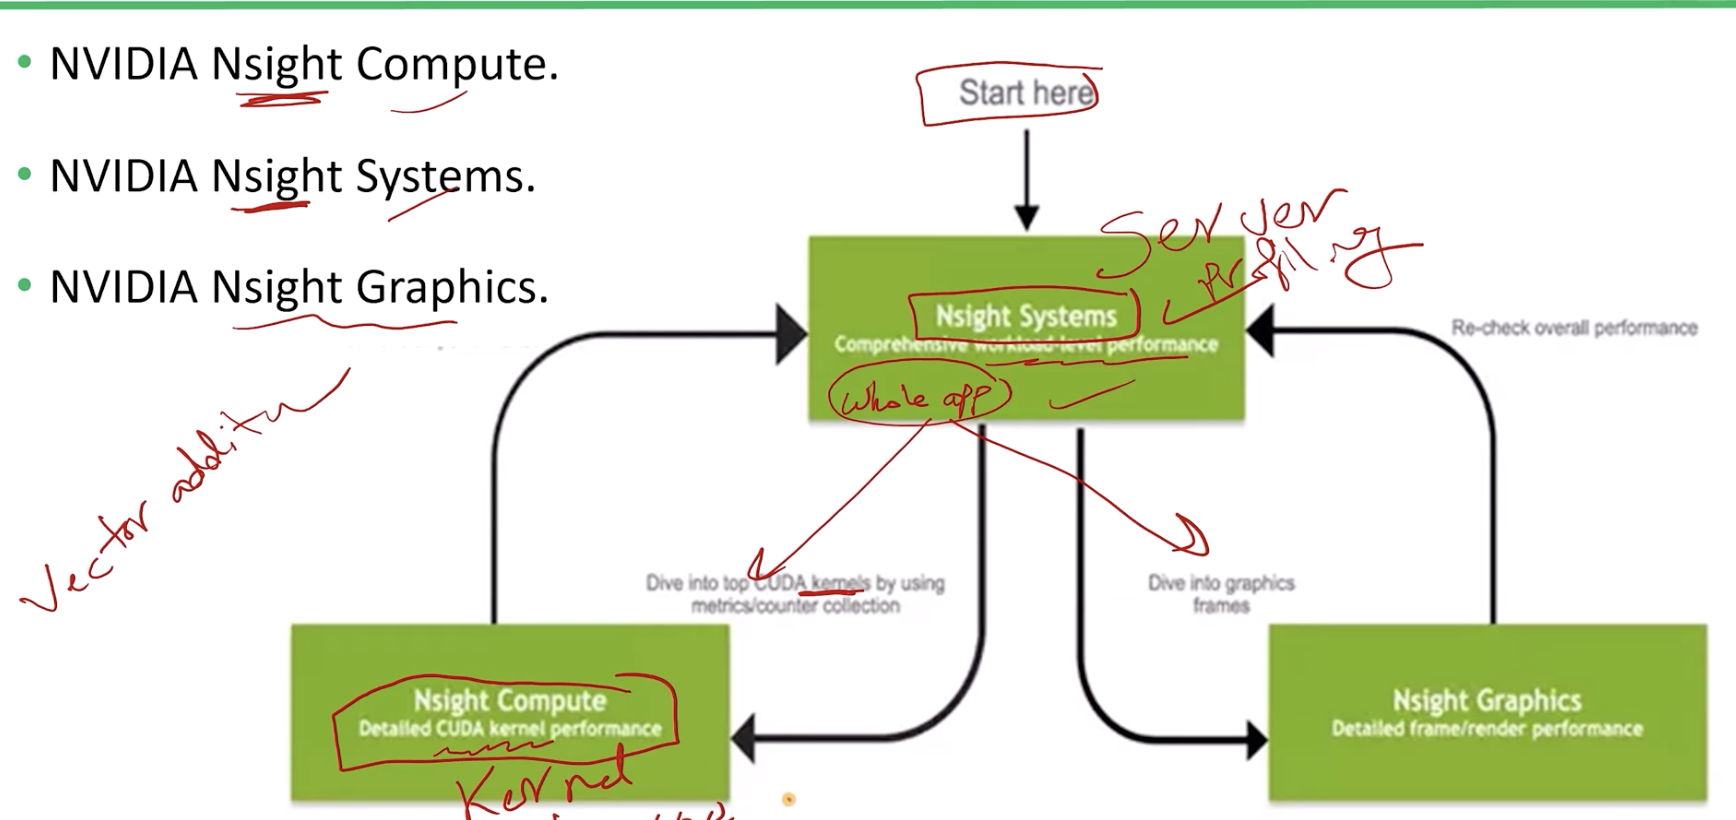
\includegraphics[width=0.75\linewidth]{resources/cuda-099.png}
    \caption{}
    \label{fig:placeholder}
\end{figure}

本章不解释所有这些工具，只专注于 Nsight 套件中三个最重要的工具：Nsight Compute、Nsight Systems 和 Nsight Graphics。这张图解释了这三个工具之间的关系。如图所示，该图从 Nsight Systems 开始，它相对于其他两个工具是外层的，这表明该工具更适合将应用程序作为一个整体来检查，而不是专注于单个核函数。这个工具即 Nsight Systems 被推荐给开发者，用于对其应用程序性能进行全系统范围的分析。当考虑到一个应用程序可能包含多个核函数，而不仅仅是一个时，这种区别就变得明显了。该工具可以可视化 CPU 到 GPU 的交互使用情况，以及 CUDA Runtime API 的性能，还能分析多节点工作负载。这就是为什么可以说 Nsight Systems 是一个服务器端分析工具，而不是客户端分析工具。这个工具就是前文分析向量加法应用程序时演示过的同一个工具。

然后为了对应用程序或工作负载中的每个核函数进行更细致的检查，Nsight Compute 是首选工具。它提供了大量针对每个核函数的详细见解和度量指标，包括全局内存、缓存、SM。甚至深入到 SM 内每个独立单元的度量指标，可用的度量指标超过 10 万个。

Nsight Graphics 提供有关图形帧和渲染性能的详细度量指标，专为图形应用程序分析和剖析的需求而定制。最后，当涉及到以图形为中心的应用程序时，Nsight Graphics 是该领域的专业工具。

在结束本章之前，留一个重要的提示。本课程中的分析重点将完全集中在 Nsight Compute 工具的使用上，可能还会涉及 Nsight Systems。
